\section{Schaltalgebra}
\subsection{Rechenregeln}
	\begin{tabular}{llll}
		Verkn"upfung mit 0 & $ a \vee 0 = a $ & $ a \wedge 0 = 0 $ & $ a \veebar 0 = a $\\
		Verkn"upfung mit 1 & $ a \vee 1 = 1 $ & $ a \wedge 1 = a $ & $ a \veebar 1 = \neg a $ \\
		Verkn. mit sich selbst & $ a \vee a = a $ & $ a \wedge a = a $ & $ a \veebar a = 0 $ \\
		Verkn. mit Inversem & $ a \vee \neg a = 1 $ & $ a \wedge \neg a = 0 $ & $ a \veebar \neg a = 1 $ \\
		\\
		Kommutativgesetz & $ a \vee b = b \vee a $ & $ a \wedge b = b \wedge a $ & $ a \veebar b = b \veebar a $\\
		Assioziativgesetz & $ (a \vee b) \vee c = a \vee (b \vee c) $ & $ (a \wedge b) \wedge c = a \wedge (b \wedge c) $ & $ (a \veebar b) \veebar c = a \veebar (b \veebar c) $ \\
		Distributivgesetz & $ a \wedge (b \vee c) = (a \wedge b) \vee (a \wedge c) $ & $ a \vee (b \wedge c) = (a \vee b) \wedge (a \vee c) $ & $ a \wedge (b \veebar c) = (a \wedge b) \veebar (a \wedge c) $ \\	
		\end{tabular}
\subsection{Vereinfachungen}
\begin{tabular}{llll}
	$ a \vee (a \wedge b) = a $ &
	$ a \wedge (a \vee b) = a $ &
	$ (a \vee !b) \wedge b = a \wedge b $ &
	$ (a \wedge b) \vee (a \wedge !b) = a $\\
	$ (a \wedge !b) \vee b = a \vee b $ &
	$ (a \wedge !b) \not= b = a \vee b $ &
	$ (a \not= !b) \wedge = a \wedge b $ &
	$ (a \vee b) \wedge (a \vee !b) = a $\\
\end{tabular}

\subsection{Shannon und DeMorgan}
	\begin{tabular}{lll}
	Ursprungsschaltung: & Shannon & DeMorgan\\
		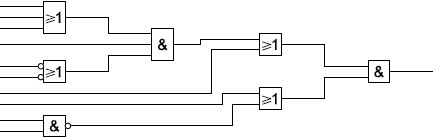
\includegraphics[width=0.3\textwidth]{pics/shanonursprung} & 
		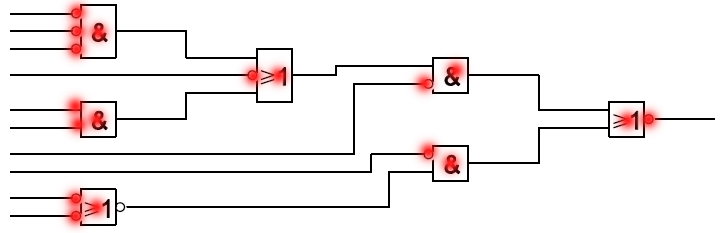
\includegraphics[width=0.3\textwidth]{pics/shanonende} &
		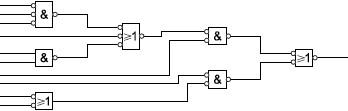
\includegraphics[width=0.3\textwidth]{pics/demorganende}\\
	\end{tabular}


\subsection{Wahrheitstabelle, KDNF, KKNF, Y-Diagramm}
\begin{tabular}{ll}
	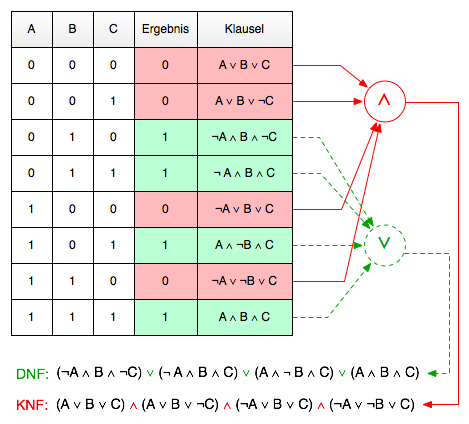
\includegraphics[width=0.5\textwidth]{pics/KNFDNF} & 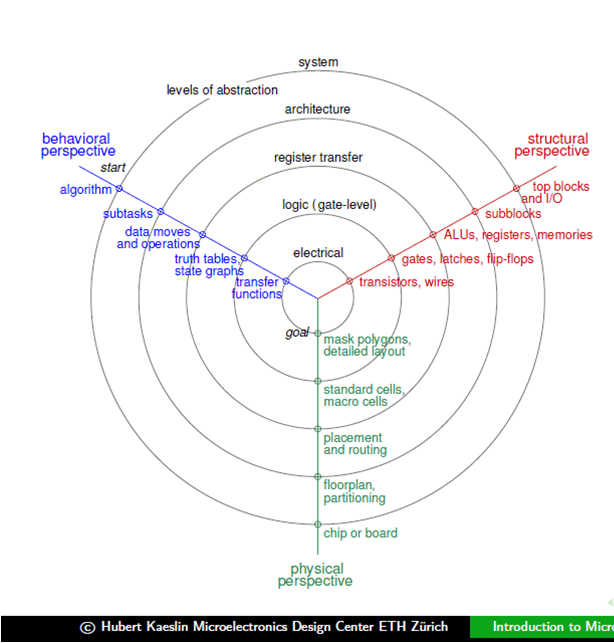
\includegraphics[width=0.5\textwidth]{pics/ydiagramm} \\
\end{tabular}
Kurzschreibweisen:\\
KNF: $ a = \&([1],[2],3) $ \\
DNF: $ b = \#([1],[3],37) $ \\
Zeugs in eckigen Klammern bedeutet don't care.
\subsection{Karnaugh-Diagramm}
\begin{tabular}{lll}
	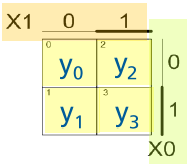
\includegraphics[width=0.2\textwidth]{pics/kv/2erKV} & 
	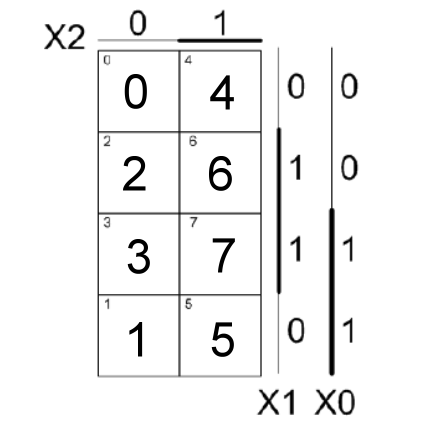
\includegraphics[width=0.2\textwidth]{pics/kv/3erKV} &
	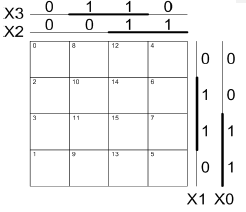
\includegraphics[width=0.3\textwidth]{pics/kv/4erKV}\\
\end{tabular}
\subsection{Arbeiten mit KV-Diagramm}
\begin{enumerate}
\setlength{\itemsep}{1pt}
  \setlength{\parskip}{0pt}
  \setlength{\parsep}{0pt}
\item Aufstellen der Wahrheitstabelle.\\
\item "Ubertragen der Werte der Wahrheitstabelle in KV Diagramm.\\
\item M"oglichst grosse Gruppen a $2^n$ Felder bilden.\\
\item
\begin{tabular}{ll}
	DNF & KNF \\
	Gruppen von Feldern mit Wert 1 oder d & Gruppen von Feldern mit Wert 0 oder d\\
	Primimplikanten: AND Verkn. & Primimplikanten: OR Verkn.\\
	OR Verkn. aller Primimpl. & AND Verkn. aller Primimpl.\\
\end{tabular}
\end{enumerate}